\documentclass[titlepage,12pt]{article}
\usepackage{graphicx,setspace,natbib,fancyvrb,geometry,rotating,capt-of}
\topmargin=-.2in\oddsidemargin=0pt\evensidemargin=0pt\textwidth=6.5in
\textheight=9in\headsep=.65in\headheight=0in

\begin{document}
\onehalfspace

\begin{singlespacing}
\title{Complete-Mix Tanks-in-Series Approach to Modeling Hydraulics of Oxidation Ponds}
\author{Cameron Bracken\\Humboldt State University\\ENGR 325}
\date{\today}
\maketitle
\newpage
\pagenumbering{roman}\pagestyle{myheadings}
\tableofcontents\addcontentsline{toc}{section}{List of Figures}
\listoffigures \addcontentsline{toc}{section}{List of Tables}
\listoftables
\newpage
\end{singlespacing}
\pagestyle{headings}\pagenumbering{arabic}

\section {Introduction}
The complete-mix tanks-in-series (CMTS) approach can be used to
model the hydraulics of oxidation ponds. The CMTS approach is a
conceptual model that is often more accurate than complex models
such as advection-dispersion.  The CMTS assumes that the total
volume of a pond can be approximated by $n$ completely mixed tanks
linked in series (Figure \ref{fig:tanks}).  The approach can be
improved by including a backwards (``recycle") flow rate between
tanks which is assumed to be a be a fraction of the overall flow
rate (Finney 2006).

Assuming a first-order reaction rate, an $n$ tank system can be
represented by (Finney 2006)

\begin{eqnarray}
-\left(\frac{Q+Q_r}{V}+k\right)c_1+\frac{Q_r}{V}c_2 & = &
\frac{-Qc_{in}}{V}
\mbox{ for tank 1} \nonumber \\
\left(\frac{Q+Q_r}{V}\right)c_{i-1}-\left[\left(\frac{Q+2Q_r}{V}\right)+k\right]c_i
& = & 0
\mbox{ for tanks } 2,3,\ldots,n-1\\
\left(\frac{Q+Q_r}{V}\right)c_{n-1}-\left[\left(\frac{Q+Q_r}{V}\right)+k\right]c_n
& = &0 \mbox{ for tank } n \nonumber
\end{eqnarray}
\begin{singlespacing}
where
\begin{center}
\begin{tabular}{rcl}
$Q$&=&influent flow rate (m$^3$/day)\\
$Q_r$&=&recycle flow rate (m$^3$)\\
$V$ &=&tank or compartment volume (m$^3$)\\
$k$&=&first order reaction rate constant (day$^-1$)\\
$c_{in}$&=&influent pollutant concentration (mg/l)\\
$c_{i}$&=&pollutant concentration in conceptual tank $i$ (mg/l)
\end{tabular}
\end{center}
\end{singlespacing}
\begin{figure}[h]\label{fig:tanks}
\begin{center}
\scalebox{.6}{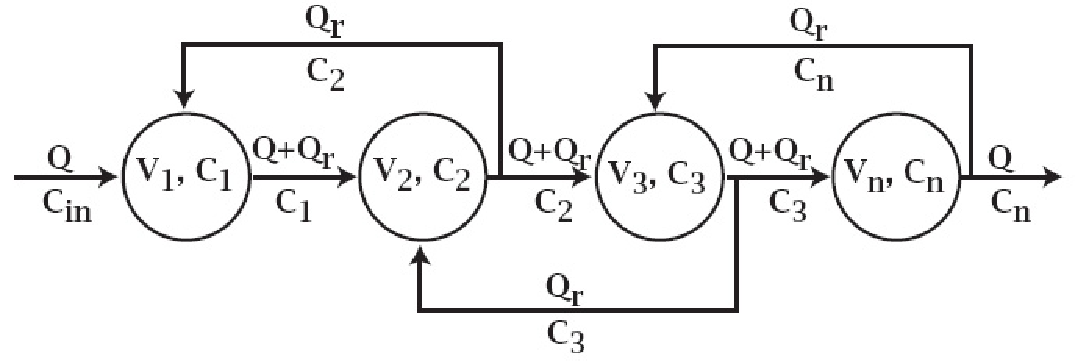
\includegraphics{tanks.pdf}} \caption{$n$ tanks in
series (Finney 2006)}
\end{center}
\end{figure}

\section{Methodology}
When expanded to fit $n$ tanks, system (1) becomes a tridiagonal
system of the general form
\begin{displaymath}
\left[
\begin{array}{cccccccc}
f_1 & g_1 & & & & & & \\
e_1 & f_2 & g_2 & & & & & \\
 & e_2 & f_3 & g_3 & & & & \\
 & & \cdot & \cdot & \cdot & & & \\
 & & & \cdot & \cdot & \cdot & & \\
 & & & & \cdot & \cdot & \cdot & \\
 & & & & e_{n-1} & f_{n-1} & g_{n-1}\\
 & & & & & e_n & f_n
\end{array}
\right] \left[
\begin{array}{c}
x_1\\
x_2\\
x_3\\
\cdot\\
\cdot\\
\cdot\\
x_{n-1}\\
x_n\\
\end{array}
\right] = \left[
\begin{array}{c}
r_1\\
r_2\\
r_3\\
\cdot\\
\cdot\\
\cdot\\
r_{n-1}\\
r_n
\end{array}
\right]
\end{displaymath}
This type of $A$\underline{$x$}=\underline{$b$} linear system can be
solved using the technique of Gauss elimination. Gauss elimination
would involve storing a large amount of empty space and carrying out
many useless computations. This problem is ideal for use with the
Gauss-Seidell (G-S) method. The G-S method is efficient in terms of
speed and memory when systems involve large numbers of zero terms.
In cases like these each equation as well as the G-S algorithm can
be can be hard-wired into the program for increased efficiency
(Chapra et al. 286-289).

The general algorithm for the G-S method with relaxation is
\begin{equation}
x_i^{(k+1)}=x_i^{(k)}+\omega
\left[\left(b_i-\sum^{i-1}_{j=1}a_{ij}x_{j}^{(k+1)}-\sum^n_{j=i}a_{ij}x_{j}^{(k)}\right)/a_{ii}\right]
\end{equation}
Where $x^{(k)}$ denotes the solution at the $k^{th}$ iteration and
$\omega$ is the relaxation factor ($0<\omega<2$) that affects the
convergence of the rate of the solution . If $\omega<1$ then the
convergence rate is underrelaxed. If $\omega>1$ then the convergence
rate is overrelaxed.  There exists a value of $\omega$ for which the
solution will converge the fastest.

A sufficient condition to ensure convergence is diagonal dominance
\begin{equation}
|a_{ii}|>\mathop{\sum^n_{j=1}}_{j\neq i}|a_{ij}|
\end{equation}
Equation (3) states that for each row the absolute value of the
diagonal element must be greater than the sum of the absolute value
of the off diagonal elements to ensure convergence (Figure
\ref{fig:diagdom}). The convergence speed of the solution is
directly related to the degree of diagonal dominance, however, the
solution may still converge if this criterion is not satisfied
(Finney 2006).

\begin{figure}[h] \label{fig:diagdom}
\begin{center}
\begin{Verbatim}[frame=single]
  do i=1,ntanks
    offdiagsum=0
    offdiagsum=sum(abs(A(i,1:ntanks)))-abs(A(i,i))
    if(offdiagsum>abs(A(i,i)))then
      write(*,*)"Answer may not converge."
    end if
  end do
\end{Verbatim}
\caption{Test for diagonal dominance}
\end{center}
\end{figure}

\break Program \verb CMTS  (Appendix A) does not utilize the full
benefits of the G-S method. Program \verb CMTS  uses the coefficient
matrix $A$ augmented with the right hand side vector \underline{$b$}
as [A$|$\underline{b}]. Storing a whole coefficient matrix is
inefficient but the calculations for this lab are not
computationally intensive. In this case the speed of the procedure
is not noticeably slowed. The G-S method is carried out within the
main program (Figure 3).

\begin{figure}[h] \label{fig:GS}
\begin{center}
\begin{Verbatim}[frame=single]
  do
    itr=itr+1
    done=0
    do i=1,ntanks
      check=0
      check=x(i)
      x(i)=x(i)+w*((AB(i,ntanks+1)-sum(AB(i,1:i-1)*x(1:i-1))&
                   -sum(AB(i,i:ntanks)*x(i:ntanks)))/AB(i,i))
      if(abs(check-x(i))<eps)then
        done=done+1
      end if
    end do
    if(stopping criteria met)then
      exit
    end if
  end do
\end{Verbatim}
\caption{Gauss-Seidell algorithm}
\end{center}
\end{figure}

The first stopping criterion for this method is a max iteration
test.  A high relaxation factor can cause the number of iterations
to be very high. The second stopping criterion is and a solution
found test
\begin{equation}
|x_i^{(k)}-x_i^{(k+1)}|<\varepsilon
\end{equation}
This method tests the solution element by element for increased
accuracy (Figure 4).

\begin{figure}[h] \label{fig:solution}
\begin{center}
\begin{Verbatim}[frame=single]
  if(abs(check-x(i))<eps)then
    done=done+1
  end if
  if(done==ntanks)then
    write(*,*)"Solution found"
    exit
  end if
\end{Verbatim}
\caption{Solution found test}
\end{center}
\end{figure}

\section{Application}
The concentration in each ``tank" is determined from various
parameters which are known in the problem (Table 1).

\begin{table}[h]
\begin{center}
\caption{Parameters associated with determining concentration
values}
% Table generated by Excel2LaTeX from sheet 'Sheet1'
\begin{tabular}{|l|l|l|}
\hline
{\bf Parameter} & {\bf Variable} & {\bf Value} \\
\hline
Influent flow rate  &        $Q$ &      10000 \\
\hline
Recycle flow rate &      $Q_r$ &      .2$Q$ \\
\hline
Tank or compartment volume &        $V$ & 50000 m$^3$ \\
\hline
First order reaction rate constant &        $k$ &  0.093/day \\
\hline
Influent pollutant concentration &   $c_{in}$ &    30 mg/l \\
\hline
Stopping tolerance  & $\varepsilon$ &    0.00001 \\
\hline
Relaxation factor &   $\omega$ &        1.0 \\
\hline
\end{tabular}
\end{center}
\end{table}

Each parameter can be varied to determine the sensitivity of the
solution

\begin{table}[h]
\begin{center}
\caption{Variation of parameters}
\begin{tabular}{|c|r|l|l|l|}
\hline
{\bf Run \#} & {\bf Variable} & {\bf Initial value} & {\bf New value} & {\bf Variation} \\
\hline
         1 &        $Q$ &      10000 &      11000 &        10\% \\

         2 &            &            &       9000 &       -10\% \\
\hline
         3 &      $Q_r$ &      .2$Q$ &     .22$Q$ &        10\% \\

         4 &            &            &     .18$Q$ &       -10\% \\
\hline
         5 &        $V$ & 50000 m$^3$ &      55000 &        10\% \\

         6 &            &            &      45000 &       -10\% \\
\hline
         7 &        $k$ &  0.093/day &     0.1023 &        10\% \\

         8 &            &            &     0.0837 &       -10\% \\
\hline
         9 &   $c_{in}$ &    30 mg/l &         30 &        10\% \\

        10 &            &            &         27 &       -10\% \\
\hline
        11 & $\varepsilon$ &    0.00001 &   0.000011 &        10\% \\

        12 &            &            &   0.000009 &       -10\% \\
\hline
\end{tabular}
\end{center}
\end{table}
\break
\section{Results}
Using the suggested value of 5 tanks, program \verb CMTS  gives
\begin{displaymath}
c =\left[
\begin{array}{ccccc}
27.03 & 24.77 & 22.70 & 20.83 & 19.34
\end{array}
\right]^T \mathrm{(mg/l)}
\end{displaymath}

The final value of the concentration ($c_{n}$) is higher than the
observed value of 19 mg/l.  A higher number of tanks must be tried
using trial and error to find a $c_{n}$ that matches the observed
value (Table 3).  18 iterations gives the closest $c_n$ to the
observed value 19 mg/l.
\begin{table}[h]
\begin{center}
\caption{Determining optimal number of tanks}
% Table generated by Excel2LaTeX from sheet 'Sheet1'
\begin{tabular}{|c|c|}
\hline
{\bf \# of Tanks} & {\bf $c_n$} \\
\hline
         5 &      19.34 \\
\hline
        10 &      19.11 \\
\hline
        15 &      19.03 \\
\hline
        16 &      19.01 \\
\hline
        17 &      19.01 \\
\hline
        18 &      19.00 \\
\hline
\end{tabular}
\end{center}
\end{table}

The sensitivity analysis reveals how $c_n$ changes with the
variation of parameters (all values found using
\underline{$c$}$_{initial}$=30, $n$=18 tanks, $\omega$=1) (Table 4).
The most influential parameter,$c_{in}$, causes a direct variation
in $c_n$. $Q_r$ and $\varepsilon$ cause the least variation in
$c_n$.

\begin{table}[h]
\begin{center}
\caption{Sensitivity analysis}
% Table generated by Excel2LaTeX from sheet 'Sheet2'
\begin{tabular}{|c|r|l|l|c|c|l|}
\hline
{\bf Run \#} & {\bf Variable} & {\bf New value} & {\bf Variation} & {\bf $c_n$} & {\bf $\Delta c_n$} & {\bf \# iterations} \\
\hline
         1 &        $Q$ &      11000 &        10\% &      19.79 &      4.16\% &         22 \\

         2 &            &       9000 &       -10\% &      18.08 &     -4.84\% &         22 \\
\hline
         3 &      $Q_r$ &     .22$Q$ &        10\% &      19.00 &      0.00\% &         24 \\

         4 &            &     .18$Q$ &       -10\% &      18.99 &     -0.05\% &         21 \\
\hline
         5 &        $V$ &      55000 &        10\% &      18.16 &     -4.42\% &         22 \\

         6 &            &      45000 &       -10\% &      19.87 &      4.58\% &         22 \\
\hline
         7 &        $k$ &     0.1023 &        10\% &      18.17 &     -4.37\% &         22 \\

         8 &            &     0.0837 &       -10\% &      19.87 &      4.58\% &         22 \\
\hline
         9 &   $c_{in}$ &         30 &        10\% &      20.90 &     10.00\% &         20 \\

        10 &            &         27 &       -10\% &      17.10 &    -10.00\% &         23 \\
\hline
        11 & $\varepsilon$ &   0.000011 &        10\% &      19.00 &      0.00\% &         22 \\

        12 &            &   0.000009 &       -10\% &      19.00 &      0.00\% &         22 \\
\hline
\end{tabular}
\end{center}
\end{table}

\break When all other parameters are held constant and $\omega$ is
allowed to vary the only effect is a change in the number of
iterations to find the solution (Table 5). The number of iterations
vary widely but the most acceptable range for the relaxation
coefficient is $.9<\omega<1.5$.  Within that range, $\omega$=1.2
yields the least iterations. A graph of the relaxation factor shows
the associated trend (Figure 5). The minimum value on the graph is
the best choice for $\omega$.
\\
\\
\begin{figure}[h]
  \begin{center}
    \scalebox{.42}{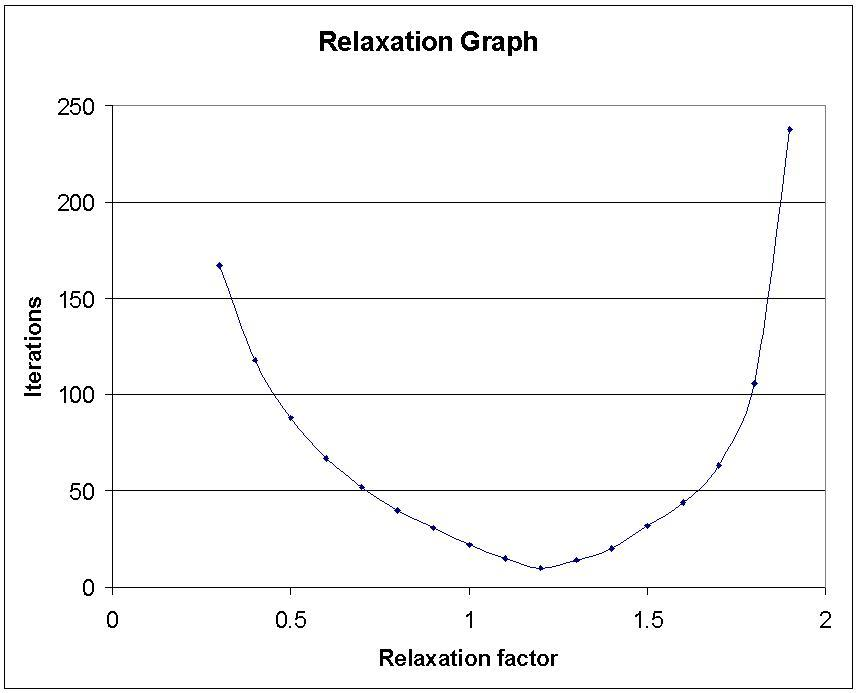
\includegraphics{relaxation.jpg}}%
    \caption{Relaxation factor vs. iteration count}
  \end{center}
\end{figure}

\begin{table}[h]
\begin{center}
\caption{Relaxation factor variation}
\begin{tabular}{|c|r|r|}
\hline
{\bf Run \#} & {\bf $\omega$} & {\bf Iterations} \\
\hline
        13 &        0.1 &        539 \\
\hline
        14 &        0.2 &        263 \\
\hline
        15 &        0.3 &        167 \\
\hline
        16 &        0.4 &        118 \\
\hline
        17 &        0.5 &         88 \\
\hline
        18 &        0.6 &         67 \\
\hline
        19 &        0.7 &         52 \\
\hline
        20 &        0.8 &         40 \\
\hline
        21 &        0.9 &         31 \\
\hline
        22 &          1 &         22 \\
\hline
        23 &        1.1 &         15 \\
\hline
        24 &        1.2 &         10 \\
\hline
        25 &        1.3 &         14 \\
\hline
        26 &        1.4 &         20 \\
\hline
        27 &        1.5 &         32 \\
\hline
        28 &        1.6 &         44 \\
\hline
        29 &        1.7 &         63 \\
\hline
        30 &        1.8 &        106 \\
\hline
        31 &        1.9 &        238 \\
\hline
        32 &          2 &      $>$5000 \\
\hline
\end{tabular}
\end{center}
\end{table}

\section{Conclusion}
The following can be concluded from the analysis:
\begin{itemize}
\item{The concentration values that 5 tanks will yield are 27.03, 24.77, 22.70, 20.83 and
19.34 mg/l respectively.}
\item{18 tanks will most closely match the observed $c_n$ value of
19 mg/l}
\item{A relaxation factor of  $\omega$=1.2 will yield the least
iterations}
\item{The most influential parameter is $c_{in}$.}
\item{Least influential parameters are $Q_r$ and $\varepsilon$.}
\end{itemize}
\break
\section{References}
Chapra, Steven, and Raymond Canale. \underline{Numerical Methods for
Engineers}. 5th ed. New York: McGraw Hill, 2006.
\\
\\
\noindent Finney,Brad. Lab 9 handout, Humboldt State University,
Spring 2006.

\appendix
\newcommand{\appsection}[1]{\let\oldthesection\thesection
  \renewcommand{\thesection}{Appendix \oldthesection}
  \section{#1}\let\thesection\oldthesection}
\appsection{\\~Source Code and Program Output} \label{sec:source}
\begin{singlespacing}
\begin{Verbatim}[frame=single]
Script started on Tue 18 Apr 2006 08:54:30 PM PDT
cwb12@ere-server:~/engr325/lab9> cat lab9.2.f90

program cmts
  implicit none
  integer::ntanks,itr,maxit,i,j
  double precision::Q,Qr,V,k,cin,w,offdiagsum,eps,check,done
  double precision,allocatable,dimension(:,:)::A,AB
  double precision,allocatable,dimension(:)::b,x
  logical::diagdom,singular
  character(len=1)::ans

  interface
    subroutine gsswap(a,neqn,diagdom,singular)
      implicit none
      integer, intent(in)::neqn
      double precision, dimension(:,:), intent(inout)::a
      logical, intent(out)::diagdom, singular
    end subroutine gsswap
  end interface

  !This program will compute the effluent concentration values of
  !a pond using the complete-mix tank-in series approach using
  !the Gauss-Seidell method to solve for the concentration values.
  !~~variable list~~
  !--input variables--
  !ntanks     =number of tanks to use as an estimate
  !Q          =influent flowrate (m^3/day)
  !Qr         =recycle flow rate (m^3/day)
  !V          =tank or compartment volume
  !k          =first order reaction rate constant (day^-1)
  !cin        =influent polution concentration
  !w          =relaxation coefficent
  !eps        =solution found tolerance
  !maxit      =maximum number of iterations
  !x          =solution vector needs initial guess
  !--output variables--
  !x          =solution vector of final concentration values
  !itr        =number of iteration carried out
  !--internal variables--
  !i,j        =loop vaiables
  !A          =holds initial coefficient matrix
  !b          =initial right hand side vector
  !ans        =answer to "do you want to continue?"

  write(*,*)"This program will compute the effluent concentration values"
  write(*,*)"of a pond using the complete-mix tank-in series approach using"
  write(*,*)"the Gauss-Seidell method to solve for the concentration values."
  write(*,*)" "
  write(*,*)"How many tanks?"
  read(*,*)ntanks
  if(ntanks<=0)then
    write(*,"(a21,i2,a6)")"Can't do operation on",ntanks," tanks"
    stop
  end if
  allocate(A(ntanks,ntanks),x(ntanks),b(ntanks),AB(ntanks,ntanks+1))
  A=0
  b=0
  Q=10000
  Qr=.2*Q
  V=50000/ntanks
  k=.093
  cin=30
  write(*,*)"Enter the relaxation coefficient 0<w<2"
  read(*,*)w
  eps=.00001
  maxit=4999
  do i=1,ntanks
    write(*,"(a28,i3)")"Enter concentration for tank",i
    read(*,*)x(i)
  end do
  A(1,1)=-((Q+Qr)/V+k)
  A(1,2)=Qr/V
  b(1)=(-Q*cin)/V
  if(ntanks>1)then
    do i=2,ntanks-1
      A(i,i-1)=(Q+Qr)/V
      A(i,i)=-((Q+2*Qr)/V+k)
      A(i,i+1)=Qr/V
    end do
    A(ntanks,ntanks-1)=(Q+Qr)/V
    A(ntanks,ntanks)=-((Q+Qr)/V+k)
  end if
  AB=A             !create augmented matrix instead of modifying originals
  AB(1:ntanks,ntanks+1)=b(1:ntanks)   !augment A with b
  write(*,*)"[A|b]="
  do i=1,ntanks
    write(*,"(a)",advance="no")"|"
    write(*,"(1000f8.3)",advance="no")(AB(i,j),j=1,ntanks+1)
    write(*,"(a)")"|"
  end do

  do i=1,ntanks
    offdiagsum=0
    offdiagsum=sum(abs(A(i,1:ntanks)))-abs(A(i,i))
    if(offdiagsum>abs(A(i,i)))then
      write(*,*)"Answer may not converge."
      write(*,*)"Continue? (y,n)"
      read(*,*)ans
      do
        if(ans=="n")then
          stop
        else if(ans/="y")then
          write(*,*)"not an option"
        else if(ans=="y")then
          exit
        end if
      end do
    end if
  end do

  call gsswap(AB,ntanks,diagdom,singular)
  !do i=1,ntanks
  !  write(*,"(a)",advance="no")"|"
  !  write(*,"(1000f8.3)",advance="no")(AB(i,j),j=1,ntanks+1)
  !  write(*,"(a)")"|"
  !end do
  if(singular)then
    write(*,*)"The coefficient matrix is singular."
    stop
  end if
  if(.not.diagdom)then
    write(*,*)"The augmented matrix is not diagonally dominant, &
               may not converge."
    write(*,*)"Continue? (y,n)"
    read(*,*)ans
    do
      if(ans=="n")then
        stop
      else if(ans/="y")then
        write(*,*)"not an option"
      else if(ans=="y")then
        exit
      end if
    end do
  end if

  !write(*,"(a11,f8.5)")"offdiagsum=",offdiagsum
  itr=0
  do
    itr=itr+1
    done=0
    do i=1,ntanks
      check=0
      check=x(i)
      x(i)=x(i)+w*((AB(i,ntanks+1)-sum(AB(i,1:i-1)*x(1:i-1))&
                     -sum(AB(i,i:ntanks)*x(i:ntanks)))/AB(i,i))
      if(abs(check-x(i))<eps)then
        done=done+1
      end if
    end do
       !write(*,*)"x="
       !do i=1,ntanks
       !  write(*,"(f10.5)")x(i)
       !end do
    if(done==ntanks)then
      write(*,*)" "
      write(*,*)"Solution found"
      write(*,*)"x="
      do i=1,ntanks
        write(*,"(f10.5)")x(i)
      end do
      exit
    else if(itr>maxit)then
      write(*,*)"No solution,max iterations exceeded"
      exit
    end if
  end do
  write(*,*)" "
  write(*,"(a12,i2,a9,f9.5)")"average for ",ntanks," tanks = "&
                                       ,sum(x(1:ntanks))/ntanks
  write(*,"(a5,i4,a12)")"took ",itr," iterations."
  write(*,*)" "
  stop
end program

cwb12@ere-server:~/engr325/lab9> ifort lab9.2.f90 gsswap.o
cwb12@ere-server:~/engr325/lab9> lab9 < values.dat
 This program will compute the effluent concentration values
 of a pond using the complete-mix tank-in series approach using
 the Gauss-Seidell method to solve for the concentration values.

 How many tanks?
 Enter the relaxation coefficient 0<w<2
Enter concentration for tank  1 Enter concentration for tank  2
Enter concentration for tank  3 Enter concentration for tank  4
Enter concentration for tank  5
 [A|b]=
|  -1.293   0.200   0.000   0.000   0.000 -30.000| |   1.200  -1.493
0.200   0.000   0.000   0.000| |   0.000   1.200  -1.493   0.200
0.000   0.000| |   0.000   0.000   1.200  -1.493   0.200   0.000| |
0.000   0.000   0.000   1.200  -1.293   0.000|

 Solution found
 x=
  27.03302
  24.76849
  22.69861
  20.83421
  19.33569

average for  5 tanks =  22.93400 took   14 iterations.

cwb12@ere-server:~/engr325/lab9> cat values.dat 5 1 30 30 30 30 30
cwb12@ere-server:~/engr325/lab9> exit

Script done on Tue 18 Apr 2006 08:55:45 PM PDT
\end{Verbatim}
\end{singlespacing}
\noindent This was typeset with \LaTeX
\end{document}
